For implementing the algorithms on big data using Hadoop and Spark, a platform was prepared which could have a deliberate setup of multiple cluster~(namenodes and worker nodes) setups containing different hardware and software resources. This could prepare a very acceptable possibility of performing performance assessment practice on different algorithms using different cluster setup. Spark and Hadoop's performance is determined by a number of parameters, including hard disk (I/O storage), CPU, memory, network bandwidth, and other software layers that are well-configured. Building a Hadoop cluster is a difficult operation that involves careful consideration of various issues, including hardware selection, cluster sizing, and configuration[hadoop cluster].

\begin{figure}[t]
   \centering
   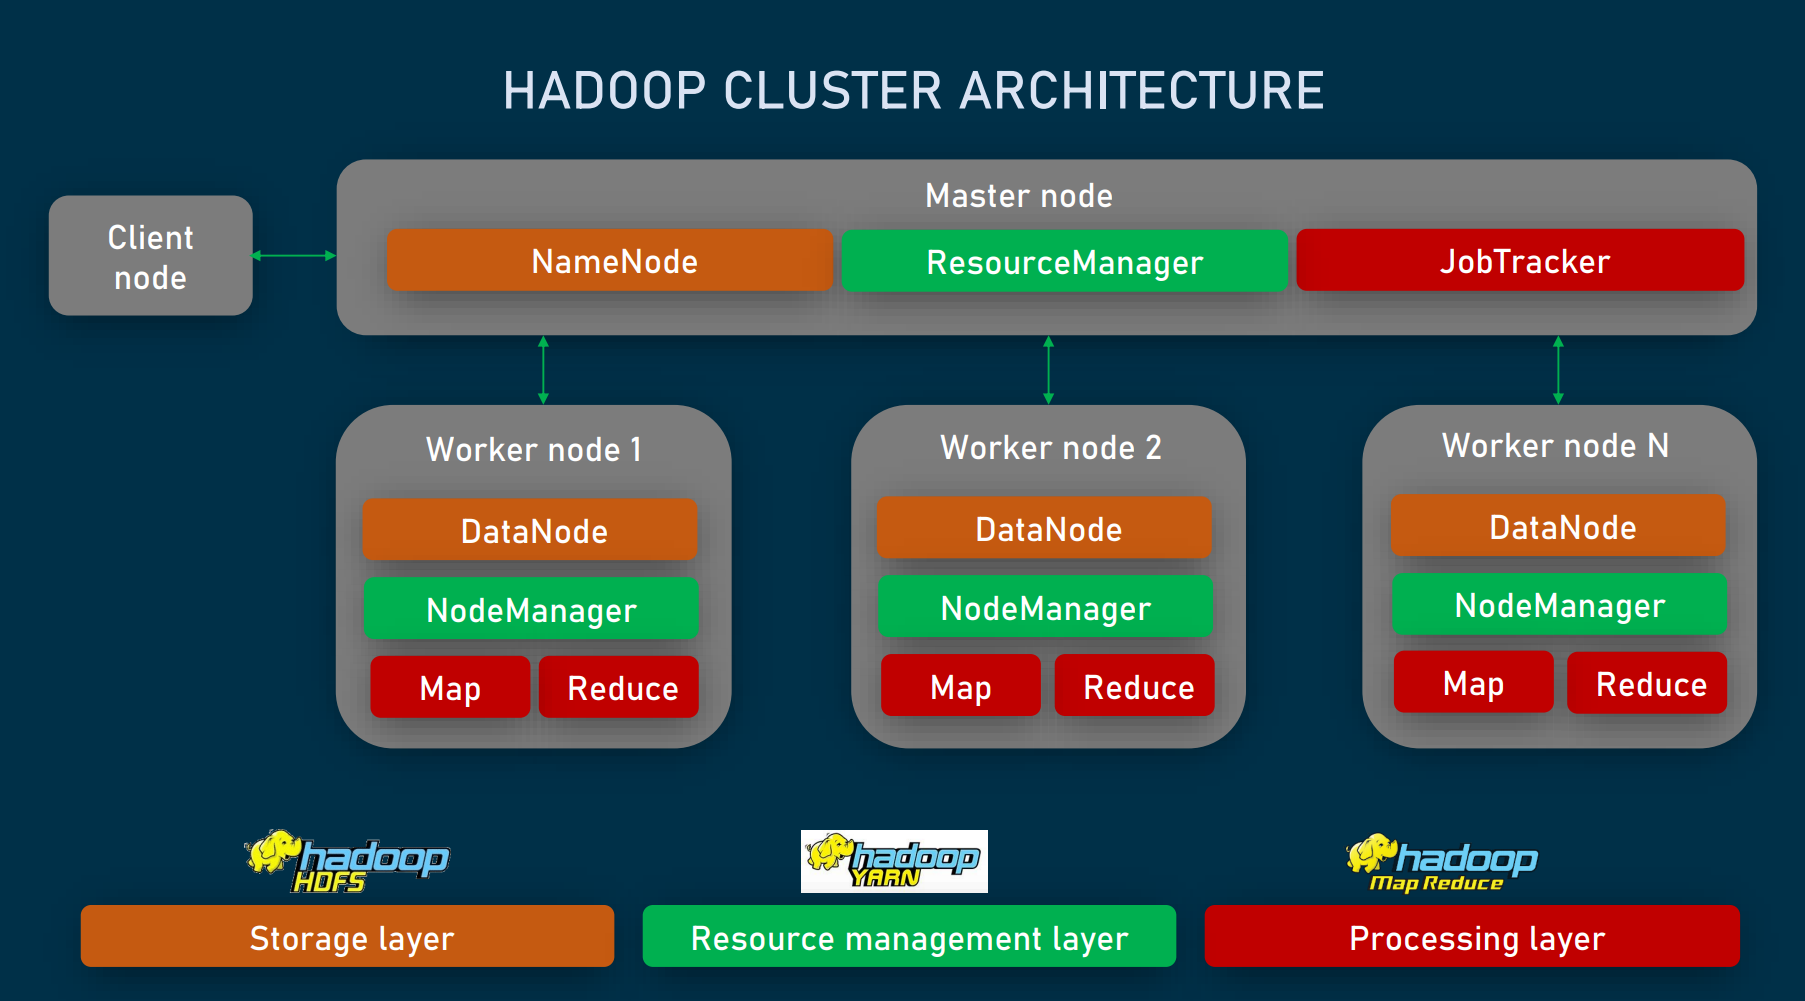
\includegraphics[width=\linewidth]{fig/hadoop_cluster.png}
    \caption{Apache Hadoop Architecture}
    \label{fig:architecture}
\end{figure}


\subsection{Experimental setup}
For this project we decided to use two different experimental setups. The primary setup contain total number of 4 nodes including one main Node and 3 data Node. The main node is named "group2" and words has been name "datanode" plus the consequent worker node order number (e.g., datanode1). All nodes had similar resources setup configuration as you can see in figure 2, there is 200~GB of HDD, 4~GB of RAM and two virtual CPU. Linux Ubuntu Forcal version 20.4 has been installed on all nodes as the operating system and Hadoop and Spark are each individually installed and configured on all nodes.
A secondary cluster configuration has also been considered which contains the same node configuration, but the total number of nodes has increased to 7 nodes including one main node and 5 worker nodes using the same naming policy.


The virtual network of the experimental setup is consisted of two networks. First one, public network and the second one group2 network which are connected together through a router.You can see the topology graph of the secondary cluster setup network on Figure~\ref{fig:topology}

\begin{figure}[t]
   \centering
   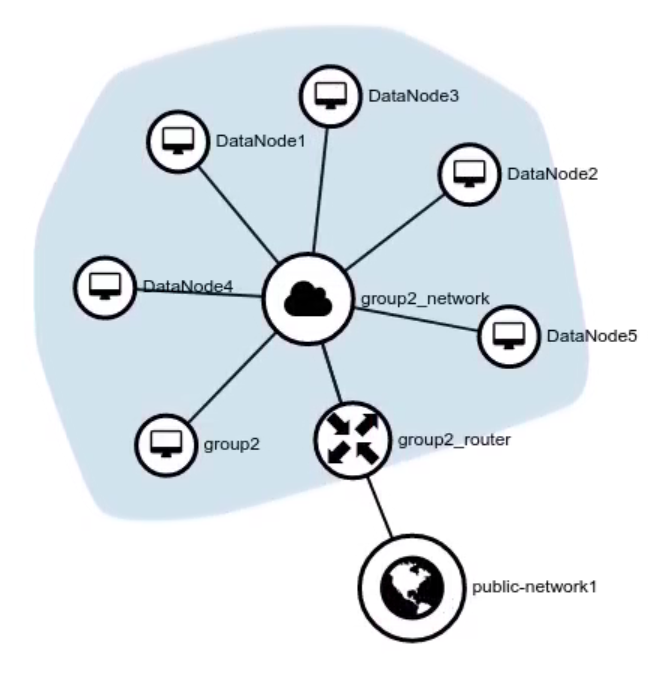
\includegraphics[width=\linewidth]{fig/NetworkTopology.png}
    \caption{Experimental Secondary Network Topology}
    \label{fig:topology}
\end{figure}


\begin{figure}
\begin{tikzpicture}
\begin{axis}[
    xlabel=YEAR,
    ylabel=Number of Reviews,
    legend entries={Maximum, Minimum, Average},
]
%The mockup experiment data is stored in a csv file, and imported here.
\addplot table [x=YEAR, y=MAX, col sep=comma] {data/reviews_month.csv};
\addplot table [x=YEAR, y=MIN, col sep=comma] {data/reviews_month.csv};
\addplot table [x=YEAR, y=AVERAGE, col sep=comma] {data/reviews_month.csv};
\end{axis}
\end{tikzpicture}
\caption{A graph showing latency and throughput of a baseline and optimized implementation. The axes show latency in milliseconds, and throughput in thousand operations per second. Data is made up.}
\label{fig:graph}
\end{figure}
